% !TeX encoding = UTF-8
% !TeX spellcheck = pt_BR

\bookmark[page=3,level=0]{Ficha Catalográfica}

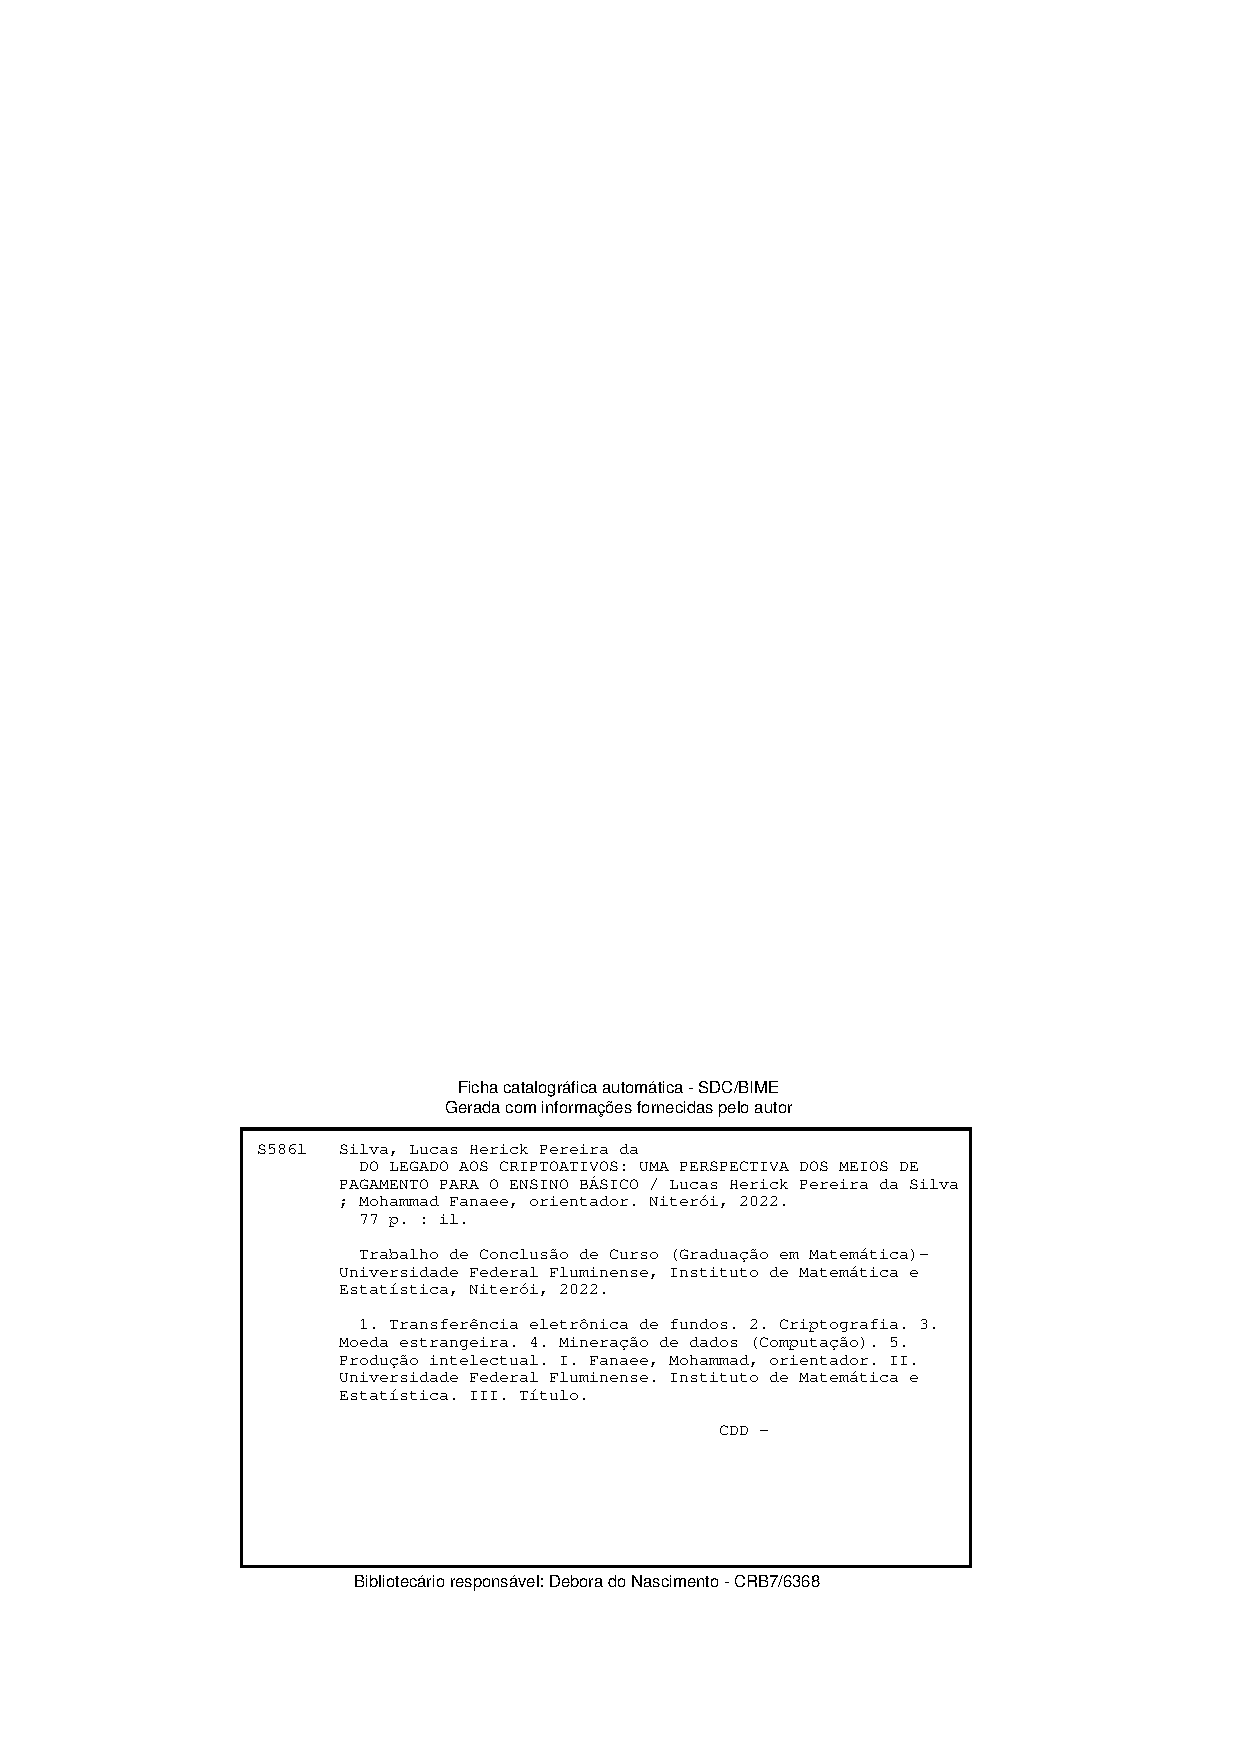
\includepdf{./ficha_cat/ficha_cat}


%\noindent\rule{\linewidth}{0.5mm}
%Folha reservada para a ficha catalográfica\\
%Gerar o arquivo aqui: \url{https://bibliotecas.uff.br/bime/fichacatalografica/}\\
%\rule{\linewidth}{0.5mm}
%
%Dados a serem inseridos no sistema: 
%
%Dados do Autor
%\begin{itemize}
%	
%	\item \fbox{Nome e sobrenomes do meio:} 
%	Lucas Herick Pereira da 
%	
%	\item \fbox{Último sobrenome:}
%	Silva
%\end{itemize}
%
%Dados do Trabalho
%\begin{itemize}
%\item \fbox{Título do trabalho:}Do legado aos criptoativos: uma perspectiva dos meios de pagamento para o ensino básico
%\item \fbox{Subtítulo do trabalho:}
%\item \fbox{Curso:} Graduação $ >> $ em Matemática
%\item \fbox{Ano:} 2022
%\item \fbox{O trabalho foi impresso frente e verso?} Sim/ Não \colorbox{yellow}{??}
%\item \fbox{Número de páginas:} 78p
%\item \fbox{Possui ilustração?} Sim
%\end{itemize}
%
%Dados do Orientador
%\begin{itemize}
%	\item \fbox{Nome do orientador:} Mohammad
%	\item \fbox{Sobrenome do orientador:} Fanaee
%\end{itemize}
%
%
%Assuntos:\\
%\vspace{1cm}
%\fbox{\begin{minipage}{.9\textwidth}
%		\begin{enumerate}
%			\item Transferência eletrônica de fundos
%			\item Moeda estrangeira	
%			\item Criptografia
%			\item Mineração de dados (Computação) 
%\end{enumerate}\end{minipage}}
